\begin{figure*}[t]
\centering
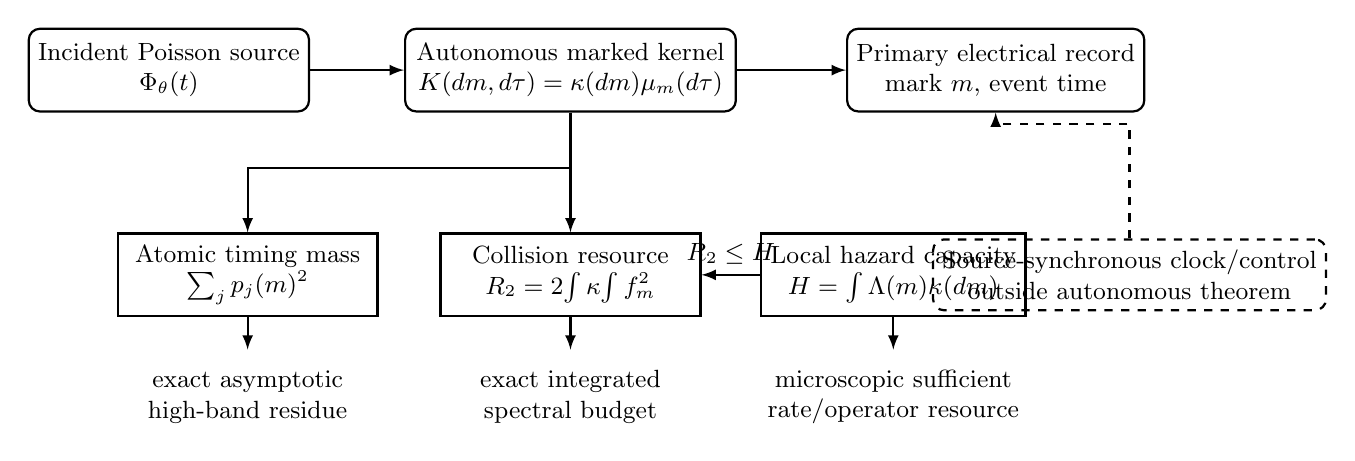
\begin{tikzpicture}[>=latex, line width=0.8pt, font=\small]
  \node[draw, rounded corners, minimum width=3.4cm, minimum height=1.05cm, align=center] (src) at (0,0)
    {Incident Poisson source\\$\Phi_\theta(t)$};
  \node[draw, rounded corners, minimum width=4.2cm, minimum height=1.05cm, align=center] (ker) at (5.1,0)
    {Autonomous marked kernel\\$K(dm,d\tau)=\kappa(dm)\mu_m(d\tau)$};
  \node[draw, rounded corners, minimum width=3.7cm, minimum height=1.05cm, align=center] (rec) at (10.5,0)
    {Primary electrical record\\mark $m$, event time};

  \draw[->] (src) -- (ker);
  \draw[->] (ker) -- (rec);

  \node[draw, minimum width=3.3cm, minimum height=1.05cm, align=center] (atom) at (1.0,-2.6)
    {Atomic timing mass\\$\sum_j p_j(m)^2$};
  \node[draw, minimum width=3.3cm, minimum height=1.05cm, align=center] (r2) at (5.1,-2.6)
    {Collision resource\\$\mathfrak R_2=2\!\int\kappa\!\int f_m^2$};
  \node[draw, minimum width=3.3cm, minimum height=1.05cm, align=center] (haz) at (9.2,-2.6)
    {Local hazard capacity\\$\mathfrak H=\int\Lambda(m)\kappa(dm)$};

  \draw[->] (ker.south) -- ++(0,-0.7) -| (atom.north);
  \draw[->] (ker.south) -- (r2.north);
  \draw[->] (haz.west) -- node[above] {$\mathfrak R_2\le\mathfrak H$} (r2.east);

  \node[align=center] at (1.0,-4.15)
    {exact asymptotic\\high-band residue};
  \node[align=center] at (5.1,-4.15)
    {exact integrated\\spectral budget};
  \node[align=center] at (9.2,-4.15)
    {microscopic sufficient\\rate/operator resource};

  \draw[->] (atom.south) -- (1.0,-3.55);
  \draw[->] (r2.south) -- (5.1,-3.55);
  \draw[->] (haz.south) -- (9.2,-3.55);

  \node[draw, dashed, rounded corners, minimum width=4.0cm, minimum height=0.9cm, align=center] (clock) at (12.2,-2.6)
    {Source-synchronous clock/control\\outside autonomous theorem};
  \draw[dashed,->] (clock.north) -- ++(0,1.45) -| (rec.south);
\end{tikzpicture}
\caption{Resource hierarchy for the autonomous marked-event theorem. The per-photon kernel maps an incident photon into a primary electrical mark and registration delay. Atomic timing mass controls the exact asymptotic flat-band residue; the capture-weighted collision intensity $\mathfrak R_2$ fixes the integrated transfer spectrum; and a capture-weighted local hazard capacity $\mathfrak H$ supplies a microscopic sufficient bound. An external source-synchronous temporal reference is a separate resource and lies outside the autonomous theorem.}
\label{fig:resourceHierarchy}
\end{figure*}
